% Drawing 156-2/01-2 -- folder 156-2, batch 01, archive page 12 (PDF page 13).
% Transcription: croquis à gauche du texte : un rectangle hachuré, ses deux côtés verticaux épaissis et marqués $A \simeq B^1$ et $B \simeq B^1$, traversé d'une courbe marquée $C \simeq D^1$ ; au-dessous, « ou », un fuseau hachuré entre deux points $A$ et $B$, traversé de même. $D^1$ est écrit ainsi, là où l'on attend $B^1$
% Kind: hatched rectangle and hatched spindle, crossed by a curve. Method 2 (schematic redraw from the facsimile). Status: ok.
% Notes: Above: a hatched rectangle, its vertical sides thickened and labelled A = B^1 and B = B^1, crossed by a curve labelled C = D^1; below, a hatched spindle between the points A and B, crossed likewise. The "ou" between them is not located on the crop and left out.
% Coordinates: 1 unit = 1 mm = 1/100 of the crop width (bbox in page fractions: [0.07, 0.64, 0.65, 0.8]).
% Redrawn by Claude (claude-opus-5-5), issue #73, 2026-11-07; not checked by a human; not compiled (no TeX in the session).
% Rights: reproduces part of the work -- behind RENDER_TRANSCRIPTS, never published by itself.
\documentclass[tikz,border=3pt]{standalone}
\usepackage{amsmath,amssymb}
\usetikzlibrary{patterns,arrows.meta}
\tikzset{pencil/.style={black!45}, struck/.style={black!35}, mark/.style={circle,draw,inner sep=1.3pt}, pt/.style={circle,fill,inner sep=0.9pt}, opt/.style={circle,draw,fill=white,inner sep=1.1pt}}
\begin{document}
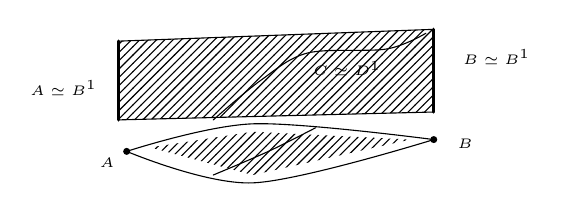
\begin{tikzpicture}[x=1mm,y=1mm,line cap=round,line join=round,font=\scriptsize]
\draw (38,-14) -- (78,-12.5);
\draw (38,-24) -- (78,-23);
\draw[very thick] (38,-14) -- (38,-24);
\draw[very thick] (78,-12.5) -- (78,-23);
\fill[pattern=north east lines] (38,-14) -- (78,-12.5) -- (78,-23) -- (38,-24) -- cycle;
\draw plot[smooth, tension=0.55] coordinates {(50,-24) (56,-19) (62,-15.5) (72,-15) (77,-13)};
\node[inner sep=1pt] at (31,-20) {\tiny $A\simeq B^1$};
\node[inner sep=1pt] at (86,-16) {\tiny $B\simeq B^1$};
\node[inner sep=1pt] at (67,-17.5) {\tiny $C\simeq D^1$};
\draw plot[smooth, tension=0.55] coordinates {(39,-28) (55,-24.5) (78,-26.5)};
\draw plot[smooth, tension=0.55] coordinates {(39,-28) (55,-32) (78,-26.5)};
\fill[pattern=north east lines] (42,-27.5) -- (55,-25.5) -- (75,-26.5) -- (55,-31) -- cycle;
\draw plot[smooth, tension=0.55] coordinates {(50,-31) (57,-28) (63,-25)};
\node[pt] at (39,-28) {};
\node[pt] at (78,-26.5) {};
\node[inner sep=1pt] at (36.5,-29.5) {\tiny $A$};
\node[inner sep=1pt] at (82,-27) {\tiny $B$};
\end{tikzpicture}
\end{document}
